\documentclass[../manuale-sviluppatore.tex]{subfiles}

\begin{document}

\subsection{Server}%
\label{sub:server}

Il backend di Stalker è costituito da un server scritto in linguaggio Java e realizzato tramite il framework \glossario{Spring Webflux}.
Il suo compito principale è quello di  soddisfare le richieste dei client che avvengono tramite chiamate di rete Http, gestire la logica di business e manipolare i modelli di dati.
Il server, inoltre, implementa gli endpoints definiti all'interno dell'\glossario{API}.

\subsubsection{Architettura backend}%
\label{architettura_backend}

L'architettura del backend, che ci è stata fortemente suggerita dal framework Spring, è monolitica.
Essa è suddivisa in strati che svolgono una funzione definita e hanno un ruolo ben distinto.
Più nello specifico, il server di Stalker ha un' architettura monolitica organizzata in 5 layer che sono così denominati:
\begin{itemize}
  \item Controller
  \item Service
  \item Model
  \item Repository
  \item Database
\end{itemize}

\begin{figure}[H]
  \centering
  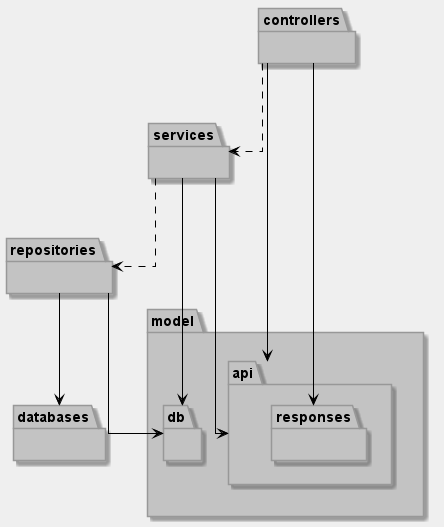
\includegraphics[width=10cm, height=8cm]{img/server-package-diagram.png}
  \caption{Diagramma dei package che illustra la struttura del server}%
   \label{fig:diagramma dei package che illustra la struttura del server}
\end{figure}

Per soddisfare le richieste dei client, le informazioni devono passare attraverso tutti gli strati.
Il controller è il layer più superficiale e che si interfaccia con le altre componenti.
Esso, inoltra la richiesta agli strati sottostanti fino allo strato di persistenza dove il server cercherà di soddisfarla.
Sia in caso di successo che di errore il server risponderà con un codice di stato Http.

Segue ora una breve descrizione di ogni strato.

\paragraph{Controller}%
\label{par:controller}

Il controller è lo strato del server che si interfaccia direttamente con i client.
Ogniqualvolta una richiesta di un client arriva al server una funzione di un controller sarà incaricata di soddisfarla.
Ciò in spring avviene grazie a delle annotazioni che effettuano il mapping tra l'endpoint e la funzione che svolgerà il ruolo di handler.

\begin{figure}[H]
  \centering
  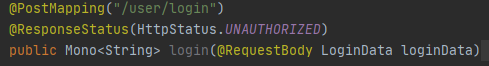
\includegraphics{img/server-controller-image.png}
  \caption{Endpoint di esempio}%
   \label{fig:immagine che illustra un endpoint di esempio}
\end{figure}

Nell'immagine soprastante si può osservare un esempio di handler implementato nel controller.
L'annotazione \textit{@PostMapping} indica che la funzione si attiverà nel caso di una chiamata post all'endpoint /user/login.
È presente, inoltre, l'annotazione \textit{@ResponseStatus} che stabilisce il tipo di codice di stato http che verrà restituito nel caso in cui la chiamata andasse a buon fine.

\paragraph{Service}%
\label{par:service}

Il service è lo strato che si occupa di gestire la logica di business.
Effettua manipolazioni sui dati sia in entrata che in uscita dal server.
Opera in due maniere opposte:
\begin{itemize}
  \item Nel caso in cui un client richieda delle informazioni, lo strato service si occupa di effettuare elaborazioni sui dati in modo che le informazioni siano accessibili ai client.
  \item Nel caso in cui un client mandi delle informazioni, lo strato service effettua le operazioni necessarie a elaborare i dati provenienti dal controller in modo che il server possa manipolarli.
\end{itemize}

\paragraph{Model}%
\label{par:model}

Il model contiene le informazioni corrispondenti ai dati presenti nel database e ai dati che i client possono inviare in formato JSON sotto forma di classi Java.
Per effettuare il mapping tra file JSON e classi Java, Spring usa di default la libreria \glossario{Jackson}.
Per realizzare, invece, il mapping delle classi Java in tabelle del database abbiamo utilizzato le \glossario{hibernate JPA annotation} che forniscono servizi di \glossario{Object-Relational-Mapping}.

\begin{figure}[H]
  \centering
  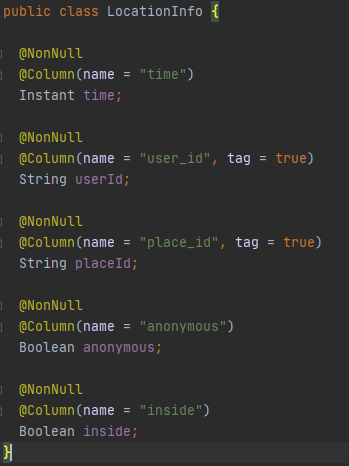
\includegraphics{img/server-hibernate-example.png}
  \caption{classe che fa uso di hibernate}%
   \label{fig:classe che fa uso di hibernate}
\end{figure}

Nella figura soprastante è presente una classe che fa uso di JPA annotations.
Quest'ultimo, infatti, tramite l'utilizzo dell'annotazione \textit{@Column} mappa ogni campo dati alla corrispettva colonna nel database.


\paragraph{Repository}%
\label{par:repository}

Lo strato repository si occupa di interagire con lo strato di persistenza e quindi di effettuare query al database.
Per interagire con il database abbiamo utilizzato il driver \glossario{R2DBC} che permette di connettere database relazionali MySQL ad API reactive.
Tramite R2DBC è possibile estendere delle interfacce e aggiungere delle annotazioni \textit{@Query} che permettono di creare query personalizzate.

\begin{figure}[H]
  \centering
  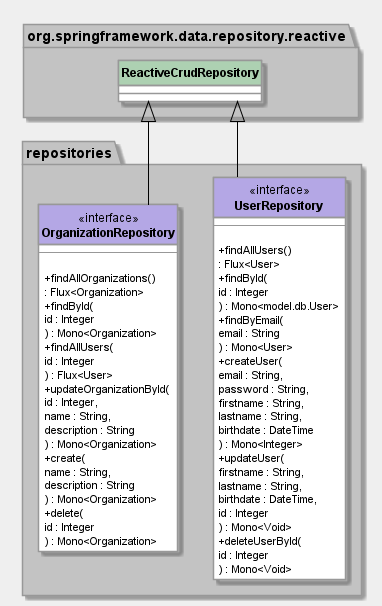
\includegraphics[width=12cm, height=15cm]{img/server-repositories-diagram.png}
  \caption{Diagramma delle classi dei repository}%
   \label{fig:diagramma delle classi dei repository}
\end{figure}

Il diagramma soprastante mostra la struttura delle interfacce del livello repositories.
Ogni metodo corrisponde ad una query sul database e restituisce Mono o Flux di oggetti del modello.
Tutte le interfacce estendono l'interfaccia ReactiveCrudRepository offerta da Spring che mediante il paradigma reactive esegue operazioni non bloccanti sul database.

\paragraph{Database}%
\label{par:database}

Lo strato di persistenza contiene i database. Il backend di Stalker è dotato di due database:
\begin{itemize}
  \item Un database mySQL per gestire i dati persistenti.
  \item Un database influxDB per gestire le timeseries, in particolare per monitorare le posizioni degli utenti.
\end{itemize}

\subparagraph{Schema relazionale database mySQL}
\label{subp:schema_relazionale_database_mysql}
Il database mySQL contiene i dati relativi agli utenti, alle organizzazioni, ai luoghi e ai ruoli ricoperti da ciascun utente nelle organizzazioni a cui è iscritto.
Nell'immagine sottostante è presente lo schema relazionale che mostra la struttura del database.
\begin{figure}[H]
  \centering
  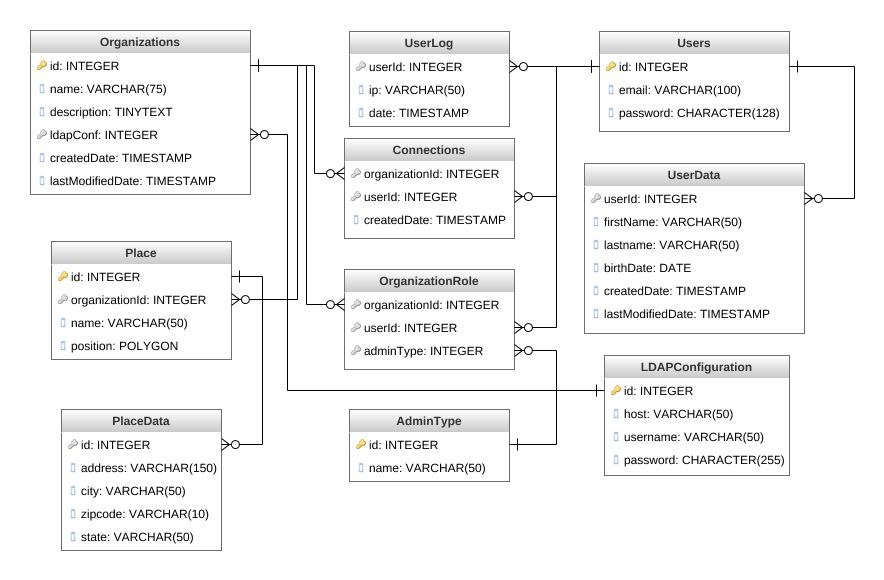
\includegraphics[width=14cm,height=10cm]{img/server-mysql-diagram.png}
  \caption{schema relazionale del database mySQL}%
   \label{fig: schema relazionale del database mySQL}
\end{figure}

\subsection{Feature d'esempio}
\label{sub:feature_d'esempio}

  \begin{figure}[H]
    \centering
    \includegraphics[width=\textwidth,height=\textheight]{img/server-influxDB-write-endpoint.png}
    \caption{diagramma delle classi d'esempio}%
     \label{fig: diagramma delle classi d'esempio}
  \end{figure}

\end{document}

